\documentclass[a4]{article}

\usepackage[left=2cm,right=2cm,top=2cm,bottom=2cm]{geometry} 

\usepackage[utf8]{inputenc}   % otra alternativa para los caracteres acentuados y la "ñ"
\usepackage[           spanish % para poder usar el español
                      ,es-tabla % para los captions de las tablas
                       ]{babel}   
\decimalpoint %para usar el punto decimal en vez de coma para los números con decimales

\usepackage{beton}
\usepackage[T1]{fontenc}

\usepackage{parskip}
\usepackage{xcolor}

\usepackage{caption}

\usepackage{enumerate} % paquete para poder personalizar fácilmente la apariencia de las listas enumerativas

\usepackage{graphicx} % figuras
\usepackage{subfigure} % subfiguras

\usepackage{amsfonts}
\usepackage{amsmath}

\definecolor{gris}{RGB}{220,220,220}
	
\usepackage{float} % para controlar la situación de los entornos flotantes

\restylefloat{figure}
\restylefloat{table} 
\setlength{\parindent}{0mm}


\usepackage[bookmarks=true,
            bookmarksnumbered=false, % true means bookmarks in 
                                     % left window are numbered                         
            bookmarksopen=false,     % true means only level 1
                                     % are displayed.
            colorlinks=true,
            allcolors=blue]{hyperref}
\definecolor{webblue}{rgb}{0, 0, 0.5}  % less intense blue


\title{AA: Práctica 3}

\author{David Cabezas Berrido}

\date{}

\begin{document}

\maketitle
\tableofcontents

\section{Clasificación de dígitos manuscritos}

\subsection{Problema}

Se nos pide clasificar imágenes de dígitos escritos a mano para
reconocer el dígito que representan (del 0 al 9). Disponemos de
ejemplos clasificados para aprender, por lo que podemos enfocarlo como
un problema de aprendizaje supervisado. Concretamente se trata de un
problema de clasificación en el que tenemos 10 clases, los dígitos del
0 al 9.

Los datos que nos proporcionan son un conjunto con 3823 instancias
para training y 1791 para test, cada instancia tiene 64 atributos que
representan el número de bits coloreados (entre 0 y 16) en cada una de
las 64 casillas que forman una cuadrícula de $8\times 8$.

Podemos visualizar ĺas instancias como matrices en lugar de vectores
para comprender mejor el formato de los datos.

\vspace{-5mm}
\begin{figure}[H]
  \centering
  \subfigure[Instancia correspondiente al 0]{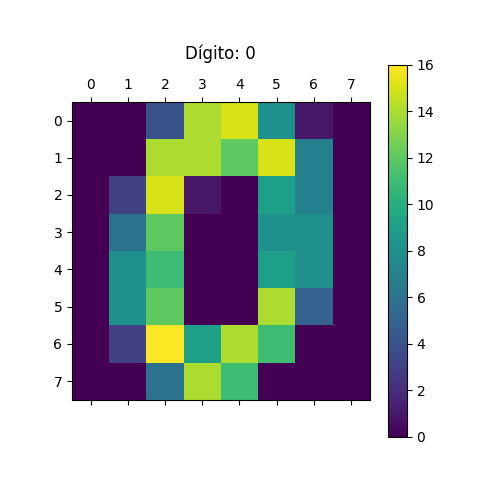
\includegraphics[width=57.5mm]{imgs/sample1.png}}
  \subfigure[Instancia correspondiente al 9]{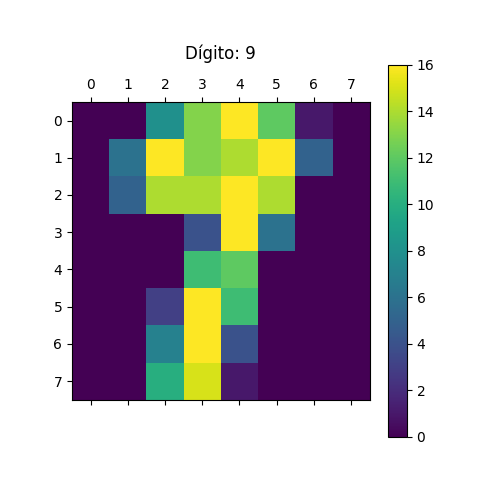
\includegraphics[width=57.5mm]{imgs/sample2.png}}
  \subfigure[Instancia correspondiente al 8]{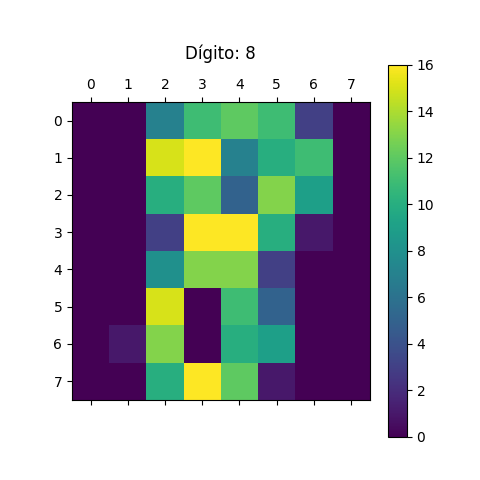
\includegraphics[width=57.5mm]{imgs/sample3.png}}
  \caption{Algunas instancias de los datos}
  \label{fig:digits-matrix}
\end{figure}

La población $X$ constituye el conjunto de vectores de 64 enteros
entre 0 y 16 que representan la cuadricula resultante de aplicar la
trasformación antes comentada.

El conjunto de clases $Y$ constituye los posibles dígitos:
0,1,2,3,4,5,6,7,8,9.

La función objetivo $f$ es la que asigna a cada vector de $X$ la clase
del dígito que representa.

\subsection{Funciones} % Quizá vaya mejor verlo junto preprocesamiento

\subsection{Conjuntos de training y test}

\subsection{Preprocesamiento}

\subsection{Métricas}

\subsection{Ajuste del modelo}

\subsection{Regularización}

\subsection{Modelos}

\subsection{Estimación de hiperparámetros y selección del modelo}

\subsection{Estimación de $E_{out}$}

\subsection{Conclusiones}

\end{document}
